130. \begin{figure}[ht!]
\center{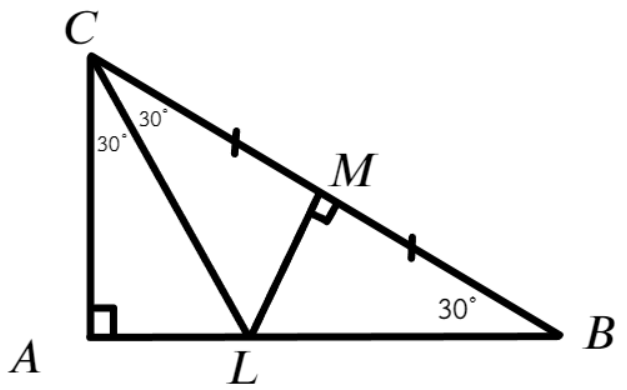
\includegraphics[scale=0.35]{g7-130.png}}
\end{figure}\\
Пусть $M$ --- середина $BC,$ тогда в треугольнике $LCB$ медиана $LM$ совпадает с высотой, значит он равнобедренный и  $CL=LB, \angle LCB=\angle B=30^\circ,$ тогда $\angle ACL=60^\circ-30^\circ=30^\circ.$ Пусть $AL=x,$ тогда по теореме о катете, лежащем напротив угла в $30^\circ,$ получим $CL=2AL=2x,\ BL=CL=2x,$ поэтому $2x-x=4,\ x=4$см. По той же теореме $ML=\cfrac{1}{2}BL=\cfrac{1}{2}\cdot4\cdot2=4$см.\\
